%TCIDATA{Version=5.00.0.2570}
%TCIDATA{LaTeXparent=0,0,Presentation-CAFE-displacement-subdoc.tex}
% $Id: Presentation-subdoc-confidentiality.tex 1765 2015-11-11 12:50:51Z lv39 $
% $URL: https://forge.cornell.edu/svn/repos/lv39_papers/BigThinkPresentations/UQAM2015/Presentation/Presentation-subdoc-confidentiality.tex $
\section{Confidentiality}

\begin{frame}
	\frametitle{Limitations of restricted data access}
	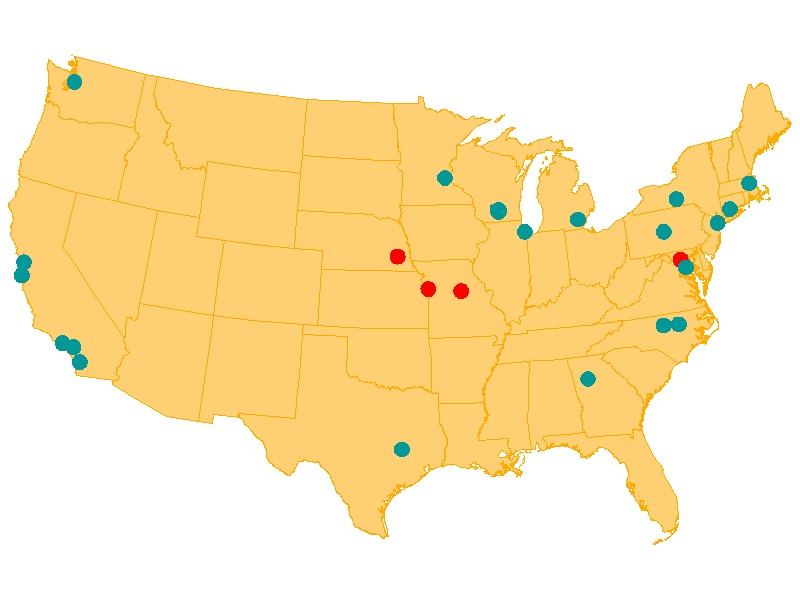
\includegraphics[width=\textwidth]{rdcmap_triad1c}
\end{frame}

\begin{frame}
	\frametitle{Limitations of restricted data access}
	\begin{block}{Users with access to (federal) confidential data in the US}
		There are {\large \textbf{21}} ({\small as of 2015-11-09}) Federal Research Data Centers (RDCs) in the US. There are approximately 300 researchers with access at any given time. (IRS: 12, BLS: 20?). There are currently {\large \textbf{6}} servers with total of 200+ CPUs available.
	\end{block}\pause
	\begin{block}{Users with access to public-use data}
		There are {\large \textbf{20-30} thousand} economists in the US. If they each have access to reasonably modern desktop, they have {\large \textbf{120k}} CPUs. Not counting compute clusters.
	\end{block}
\end{frame}

\begin{frame}
	\frametitle{Who wants to sit in this?}
	\begin{block}{UK efforts}
		\centering 
		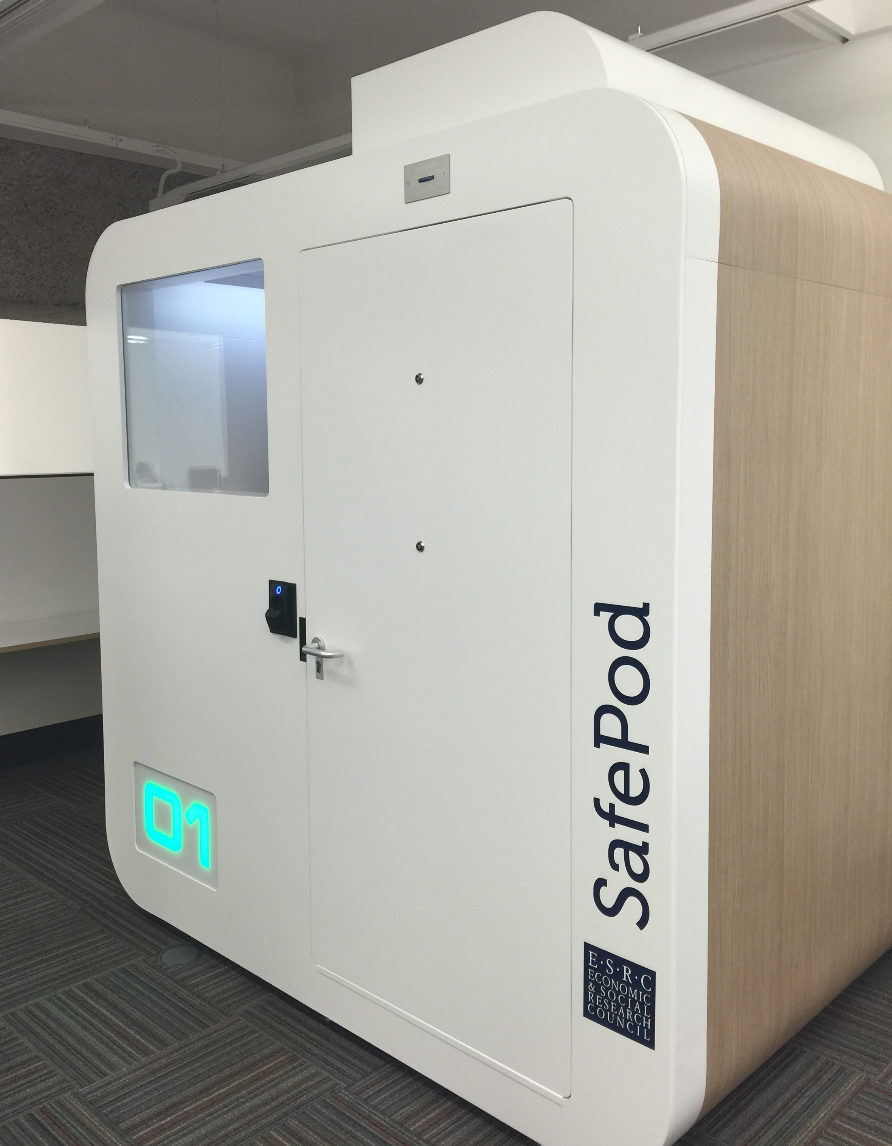
\includegraphics[height=0.8\textheight]{SafePODS}
	\end{block}
	
\end{frame}


\begin{frame}
	\frametitle{Who wants to sit in this?}
		\centering 
		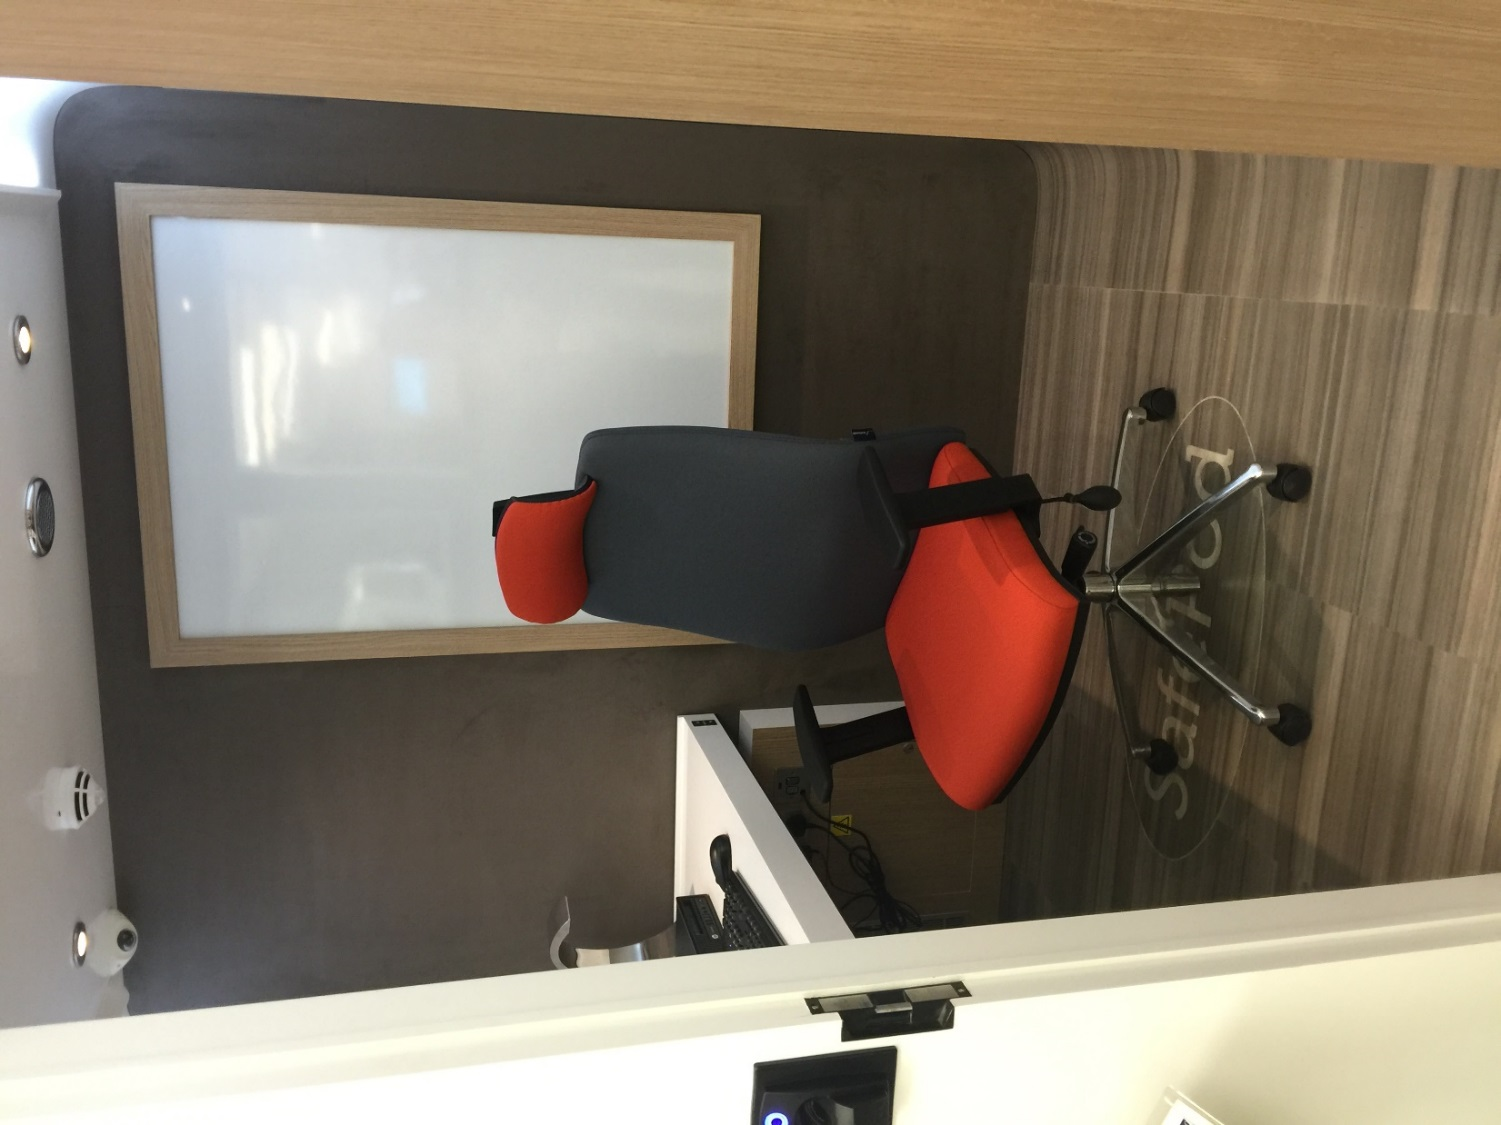
\includegraphics[height=0.6\textheight,angle=270]{SafePODS2}
		
	\tiny Src: \href{http://www1.unece.org/stat/platform/display/SDCWS15/}{Univ. Edinburgh -- Micro, remote, safe settings (safePODS) -- extending a safe setting network across a country}
\end{frame}



\begin{frame}
	\frametitle{Data liberation!}
{\Large Data curators trade off}
\begin{itemize}
	\item Providing detailed and accurate statistics 
	\item Protecting privacy and confidentiality 
\end{itemize}
\onslide<2>{\Large What is the optimal tradeoff, given the data have already been collected?}
\end{frame}

\begin{frame}
	\frametitle{Data curator strategies}
	\begin{block}{Limit access}
		\begin{itemize}
		    \item Let researchers run wild (with models)...
			\item ... and limit what can be removed (mostly adhoc)
			\item RDCs
			\item remote processing with delay and cost
		\end{itemize}
	\end{block}
	\begin{block}{Public-use files}
\begin{itemize}
	\item Disclosure limitation (aggregation, swapping, suppression, etc.)
\end{itemize}
	\end{block}
\end{frame}

\begin{frame}
	\frametitle{Some newer methods}
	\begin{block}{Multiplicative Noise Infusion}
		\begin{columns}
\begin{column}{0.7\textwidth}
	\footnotesize
\begin{equation*}
p\left( {\delta _{j}}\right) =\left\{ {{%
		\begin{array}{*{20}c} {\mbox{ }{\left( {b - \delta } \right)} \mathord{\left/ {\vphantom {{\left( {b - \delta } \right)} {\left( {b - a} \right)^2}}} \right. \kern-\nulldelimiterspace} {\left( {b - a} \right)^2},\;\delta \in \mbox{ 
				}\left[ {a,b} \right]} \\ {{\left( {b + \delta - 2} \right)} \mathord{\left/ {\vphantom {{\left( {b + \delta - 2} \right)} {\left( {b - a} \right)^2}}} \right. \kern-\nulldelimiterspace} {\left( {b - a} \right)^2},\;\delta \in \left[ {2 - b,2 - a} \right]\mbox{ }} \\ {0,\;\mbox{ otherwise }} \\ \end{array}%
				}}\right. 
\end{equation*}%
\begin{equation*}
				F\left( {\delta _{j}}\right) =\left\{ {{%
						\begin{array}{*{20}c} {\mbox{0},\;\delta < {2-b} } \\ {{\left[ {\left( {\delta + b - 2} \right)^2} \right]} \mathord{\left/ {\vphantom {{\left[ {\left( {\delta + b - 2} \right)^2} \right]} {\left[ {2\left( {b - a} \right)^2} \right]}}} \right. \kern-\nulldelimiterspace} {\left[ {2\left( {b - a} \right)^2} \right]},\;\delta \in \left[ {2 - b,2 - a} \right]\mbox{ }} \\ {\mbox{0.5}, \;\delta \in \mbox{ }\left( {2-a,a} \right)\mbox{ }} \\ {\mbox{0.5} + {\left[ {\left( {b - a} \right)^2 - \left( {b - \delta } \right)^2} \right]} \mathord{\left/ {\vphantom {{\left[ {\left( {b - a} \right)^2 - \left( {b - \delta } \right)^2} \right]} {\left[ {2\left( {b - a} \right)^2} \right]}}} \right. \kern-\nulldelimiterspace} {\left[ {2\left( {b - a} \right)^2} \right]},\;\delta \in \mbox{ }\left[ {a,b} \right]\mbox{ 
								}} \\ {\mbox{1}, \;\delta > {b} } \\ \end{array}}}\right. 
\end{equation*}%
\noindent where $a=1+{c}/{100}$ and $b=1+{d}/{100}$ are constants chosen
such that the true value is distorted by a minimum of $c$ percent and a
maximum of $d$ percent
\end{column}
\begin{column}{0.3\textwidth}
				
			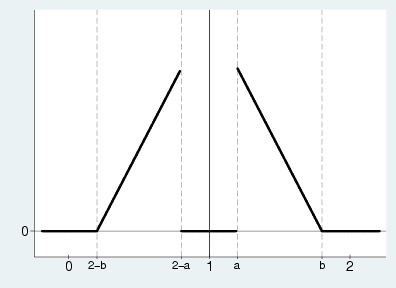
\includegraphics[width=0.9\textwidth]{fuzzfactors}
\vspace{0.5\textheight}
\end{column}	
\end{columns}
\end{block}
\end{frame}

\begin{frame}
	\frametitle{Applying noise infusion}
	\begin{block}{Quarterly Workforce Indicators}
Published value $X_{jt}^{\ast}$ computed from confidential value $X_{jt}$ as
\begin{equation}
X_{jt}^{\ast }=\delta _{j}X_{jt},  \label{eq:fuzz_totals}
\end{equation}%
	\end{block}
	See \href{https://ideas.repec.org/h/nbr/nberch/0485.html}{Abowd et al (2009)}
\end{frame}

\begin{frame}
	\frametitle{Synthetic data (Rubin, 1993; Little, 1993)}
	\begin{block}{Drawing from a posterior predictive distribution}
		\begin{itemize}
			\item[\ ] From data $\left ( X, Y ) \right )$, where $Y=\left ( Y_{obs}, Y_{nobs} \right )$
			\item[\ ] $I: i=0 \iff y \in Y_{nobs}$, 
			\item[\ ] construct PPD as $\left ( Y | X, Y_{obs}, I \right )$, and 
			\item[\ ] draw $Y^{\ast}$. 
			\item[\ ] Then release $\left ( X, Y^{\ast}_k \right )$ ($k$ partially synthetic data sets, typically $k>1$)
			\item[\ ] Similarity: $\left (X, (Y_{obs},Y_{nobs}^{\ast} ) \right )$ (multiply) imputed data
		\end{itemize}
	\end{block}
\end{frame}



\begin{frame}
	\frametitle{Examples of synthetic microdata}
	\begin{block}{SIPP Synthetic Beta}
		Survey of Income and Program Participation (SIPP) matched to administrative earnings, then synthesized
	\end{block}
	\begin{block}{Synthetic LBD (SynLBD)}
	   Longitudinal Business Database -- longitudinally linked establishment microdata -- synthesized
	\end{block}
\end{frame}

\begin{frame}
	\frametitle{Other uses of synthetic data}
	\begin{block}{American Community Survey tabulations}
		Group quarters
		\end{block}
		\begin{block}{LEHD Origin-Destination Employment Statistics (LODES)}
          Synthetic (differentially private) residence information combined with noise-protected establishment counts. (Machanavajjhala et al, 2008)
\end{block}
\end{frame}


\begin{frame}
	\begin{beamercolorbox}[sep=8pt,center]{title}
		\usebeamerfont{title} Key: analytic validity contingent on privacy protection
	\end{beamercolorbox}
	\centering \vspace{2cm}
How well does that work?
\end{frame}

\begin{frame}
	\frametitle{LODES}
	\centering
	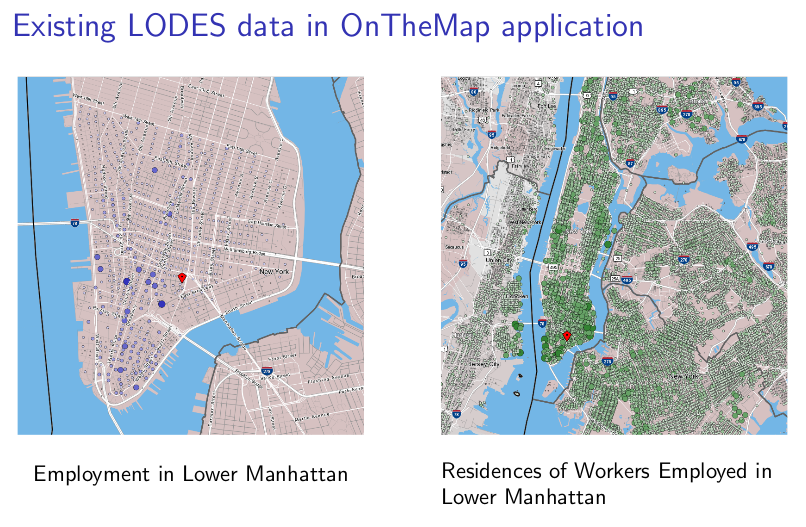
\includegraphics[width=0.9\textwidth]{sam-4}
\end{frame}


\begin{frame}
	\frametitle{Synthetic Data Server @ Cornell}
	\begin{block}{Open remote access}
		\begin{itemize}
			\item Users request account (no restrictions)
			\item Users run regression on synthetic data
			\item Users request validation against confidential data
		\end{itemize}
	\end{block}
\end{frame}

\begin{frame}
	\frametitle{Bertrand et al 2015}
	\begin{block}{From Bertrand et al (2015)}
		\centering
	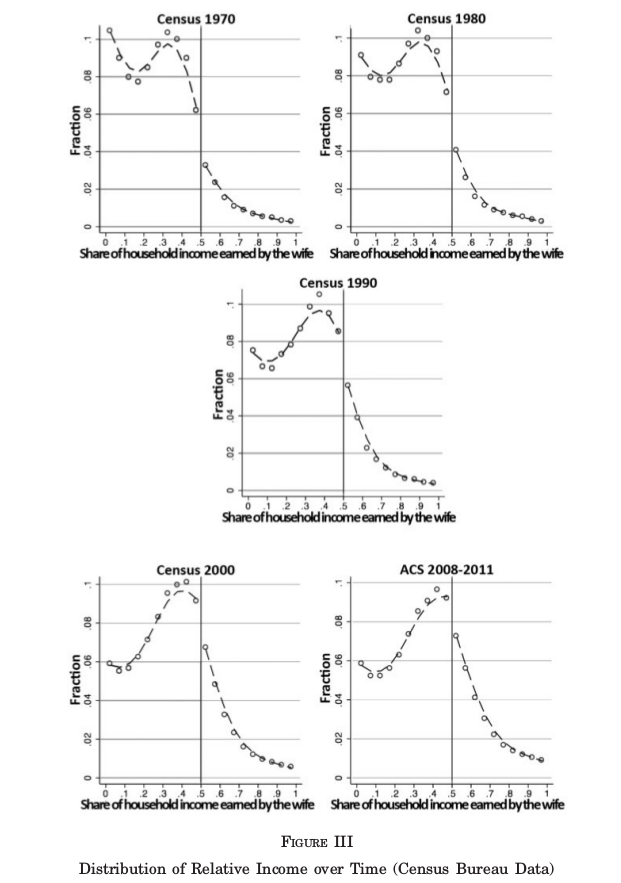
\includegraphics[width=0.5\textwidth]{Bertrand-QJE-2015-FigureIII}
\end{block}
\end{frame}



\begin{frame}
	\frametitle{Bertrand et al 2015}
	\centering
	{From Bertrand et al (2015), their Figure~I}
	\begin{tabular}{cc}
		(a) & (b)\\
		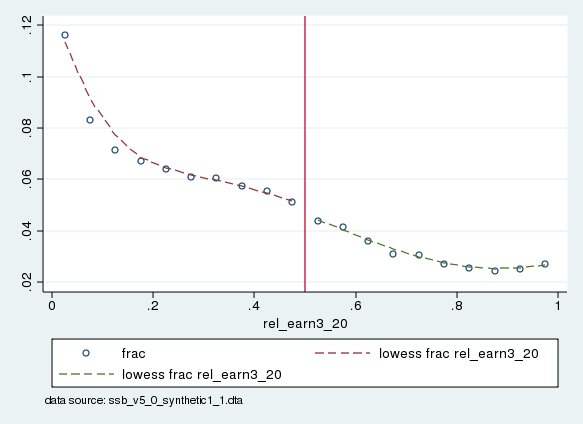
\includegraphics[width=0.4\textwidth]{jma_graph_rel_earn3_syn}&\pause
		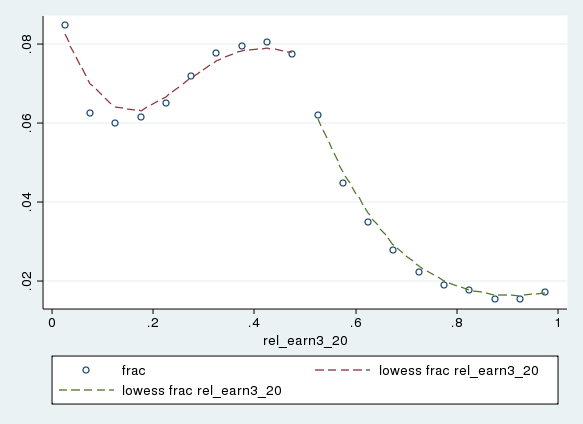
\includegraphics[width=0.4\textwidth]{jma_graph_rel_earn3}\\
	\end{tabular}
\end{frame}


\begin{frame}
	\frametitle{Synthetic data as a `blind commitment' device}
	\begin{block}{``Blind analysis: Hide results to seek the truth''}
		\href{http://www.nature.com/news/blind-analysis-hide-results-to-seek-the-truth-1.18510}{Nature, October 7, 2015}
``		\begin{quote}
			temporarily and judiciously removing data labels and altering data values to fight bias and error
		\end{quote}''
	\end{block}
	Synthetic data together with validation provides such a mechanism.
\end{frame}


\begin{frame}
	\frametitle{Bertrand et al 2015}
	\centering
	{From Bertrand et al (2015), their Figure~I}
\begin{columns}
	\begin{column}{0.5\textwidth}
		\centering
%	\begin{tabular}{p{.4\textwidth}p{.4\textwidth}}
%		(a) & (b)\\
		\only<1>{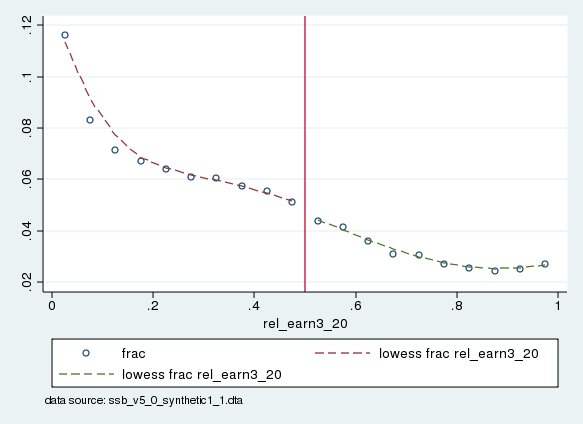
\includegraphics[width=0.95\textwidth]{jma_graph_rel_earn3_syn}}
	    \only<2>{Lifting of veil}
		\end{column}
%		&%\pause
\begin{column}{0.5\textwidth}
	\centering
		\only<2>{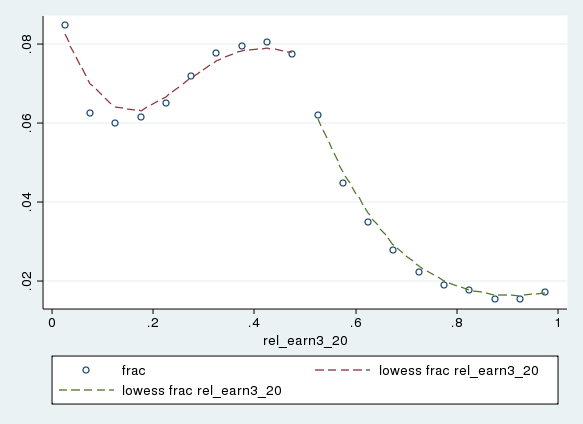
\includegraphics[width=0.95\textwidth]{jma_graph_rel_earn3}}
		\only<1>{ Blind model specification}\\

\end{column}	
%\end{tabular}
\end{columns}
\end{frame}


\begin{frame}
	\frametitle{Importance of feedback loop}
	\begin{block}{Account creation and events SDS}
		\centering
		
		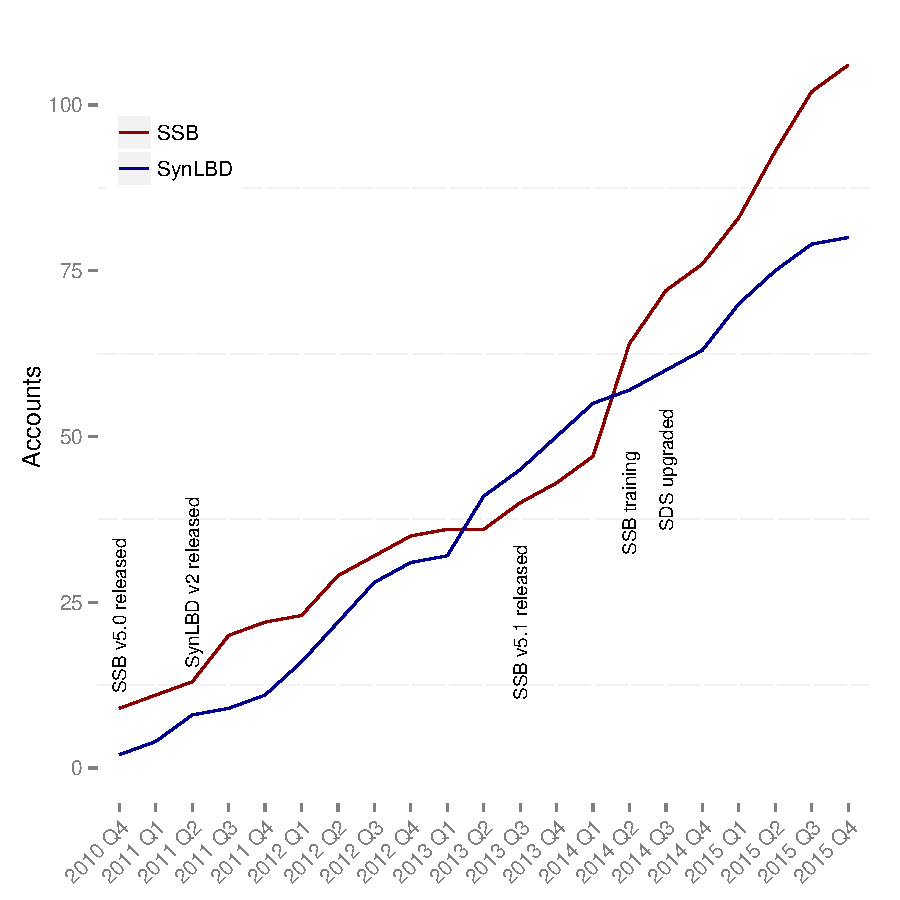
\includegraphics[width=0.6\textwidth]{report_on_SDS_2015_SOLE-accounts}
	\end{block}
\end{frame}

\begin{frame}
	\frametitle{More general validity results}
	Consider the overlap of confidence intervals $(L,U)$ for $\beta_{k,m}$ (estimated from the confidential data) and $(L^{*},U^{*})$ for $\beta_{k,m}^*$ (from the synthetic data).
	\begin{block}{Confidence interval overlap (Karr et al 2006)}
		\begin{itemize}
			\item[\ ]  Let $L^{over} = \max (L,L^{*} )$ 
			\item[\ ]  Let $U^{over} = \min (U,U^{*})$. 
			\item[\ ] Compute $J_{k,m}$ for parameter $k$ in model $m$. 
	\end{itemize}
Then the average overlap in confidence intervals 		
$$
J_{k,m}^{*} = \frac{1}{2} \left [ \frac{U^{over} - L^{over}}{U-L} + \frac{U^{over} - L^{over}}{U^*-L ^*}        \right ]
$$

We then average $J_{k,m}^{*}$ over all estimated models and parameters
\end{block}
\end{frame}


\begin{frame}
	\frametitle{Results from 3000 models and 14000 parameters}

\begin{table}[ht]
\caption{Confidence interval overlap $J_{k,m}^{*}$\label{tab:coverage}}
\centering
	\begin{tabular}{lrrrrr}
User&Request&  Mean&  75th & 90th & Max  \\
		   \hline
A    &1     & 0.160&  0.246 & 0.725& 0.889      \\%spec273
A    &2     & 0.101&  0     & 0.523& 0.924      \\%spec273
B%    &1     & 0.869&  1.000 & 1.000& 1.000      \\%spec444
C    &1     & 0.219&  0.509 & 0.725& 0.995      \\%spec527
	\end{tabular}
	
\end{table}
% Manually transcribed from email Oct 29 2015
	



\end{frame}

\begin{frame}
	\begin{beamercolorbox}[sep=8pt,center]{title}
		\usebeamerfont{title} Caution: large number of queries exhaust the ``privacy budget''
	\end{beamercolorbox}
\end{frame}
\newcommand{\M}{\mathcal{M}}
\begin{frame}[fragile]
	\frametitle{Protection against all possible queries}
	\begin{block}{Differential privacy}

					Let $\M$ be a randomized algorithm. Let $D$ and $D'$ be tables that differ in the presence of a single record (\textit{neighbors}). $\M$ satisfies $(\epsilon, \delta)$-differential privacy if for all $S \subseteq range(\M)$,
$$
			\log \frac{\Pr[\M(D) \in S]}{\Pr[\M(D') \in S] + \delta} \ \le \ \epsilon
$$

		$\delta$ allows for the ratio of probabilities to be unbounded with a small failure probability. To avoid algorithms that disclose individual records, $\delta$ should be set smaller than $1/n$. 
	\end{block}
\end{frame}


\begin{frame}
	\frametitle{Information content is limited}
	\begin{block}{Sequence of queries matters}
		\begin{itemize}
		    \item Order matters!
			\item Data custodian must decide which queries (=tables) to release first
			\item Then leave remaining privacy budget to researchers (?)
		\end{itemize}
	\end{block}
	\begin{block}{No free lunch}
         No information can be released without some privacy loss.
	\end{block}
\end{frame}


\begin{frame}
	\frametitle{Abowd and Schmutte (2014, 2015)}
\frametitle{Accuracy}
\begin{definition}[$(\protect\alpha ,\protect\beta )$-accuracy]
	\label{def:acc} A query release mechanism $M$ satisfies $(\alpha ,\beta )$%
	-accuracy for query sequence $\left\{ f_{1},f_{2},\ldots ,f_{k}\right\} \in
	\mathcal{F}^{k}$, $0<\alpha \leq 1$, and $0<\beta \leq 1$, if
	$$\min_{1\leq i\leq k}\left\{ \Pr \left[ |a_{i}-f_{i}(x)|\leq \alpha \right] \right\} \geq
	1-\beta. $$%
\end{definition}
		\end{frame}

\begin{frame}
	\frametitle{Abowd and Schmutte}
	\begin{block}{Model the demand for accuracy (social welfare function SWF)}
\centering
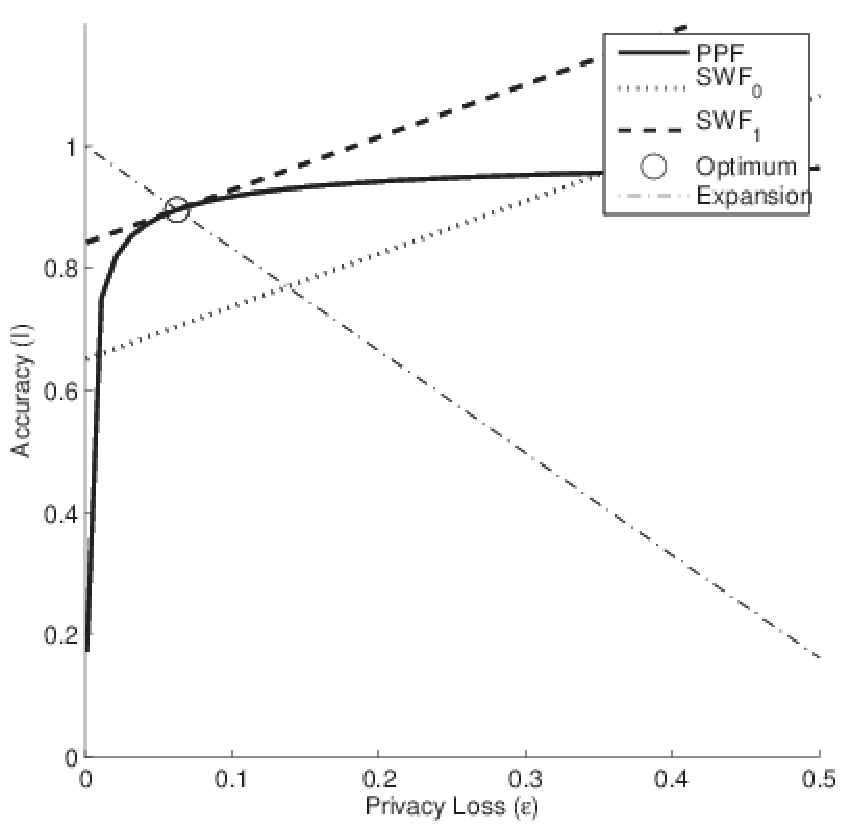
\includegraphics[width=0.6\textwidth]{plannersprob_health_complex}		
	\end{block}
\end{frame}
 \begin{frame}

 \frametitle{Technology for Anonymization}

 \textbf{Intuition:} Online Query Mechanism
 \begin{enumerate}
 	\item User sends query\vspace{.25in} 
 	\item Mechanism returns random output conditional on
 	\begin{itemize}
 		\item database
 		\item history\vspace{.25in} 
 	\end{itemize}
 	\item Use mechanisms that are provably \textit{differentially private}

 \end{enumerate}
 \end{frame}


\begin{frame}
	\frametitle{Relevancy to medical applications}
\begin{block}{Confidentiality and socio-medical data}
\begin{itemize}
	\item Restricted-access: e.g. \ac{HRS} biomarkers (same level of confidentiality as other more detailed data)
	\item Restricted remote access (remote data enclave): health insurance (``all-payer'') claims data (APCDs) [\ac{HCCI}]
	\item Trade-off: \ac{MIDUS} coarsens geography, but does not modify biomarkers
\end{itemize}

\end{block}

\end{frame}



\begin{frame}
	\frametitle{Relevancy to medical applications}\centering
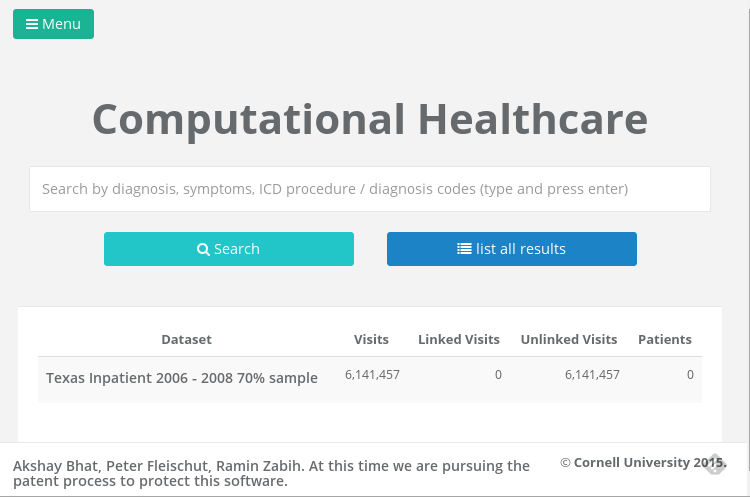
\includegraphics[width=0.8\textwidth]{Screenshot_system_20151002}
\end{frame}

\begin{frame}
	\frametitle{Relevancy to medical applications}\centering
	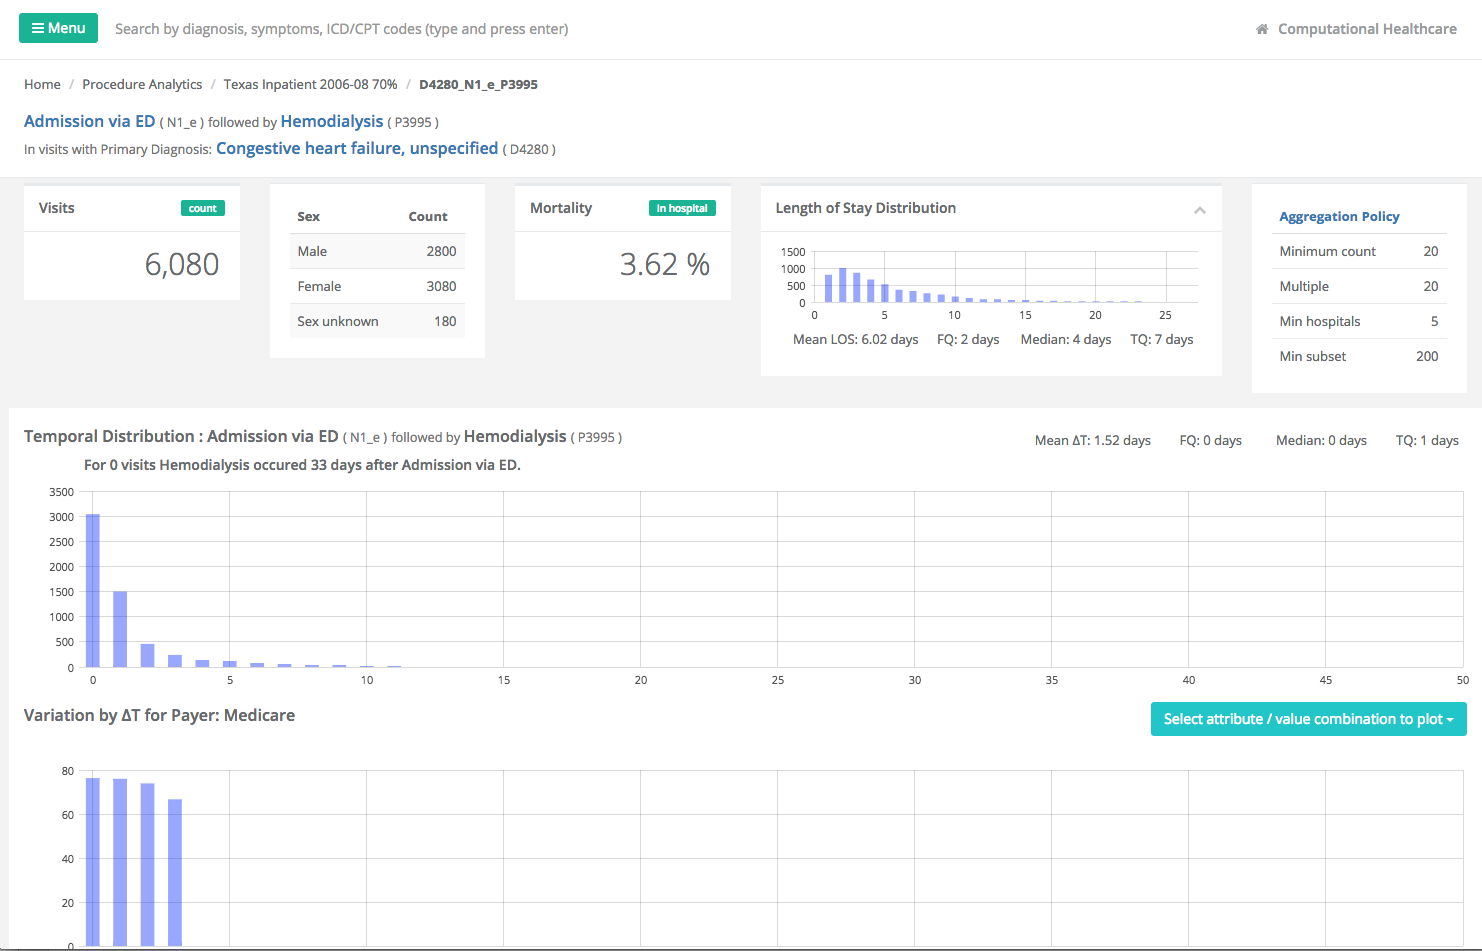
\includegraphics[width=0.8\textwidth]{Screenshot_system_20151003}
	\end{frame}

\begin{frame}
	\frametitle{Interactively exploring the technological frontier}
	\begin{block}{Active use is critical}
Provide users with an online query frontend that
interfaces directly with the confidential data, providing differentially private answers. This may still require
that all users be authorized users (TBD), and may be appropriate for certain research hospital settings.	The benefit would come from agency-signoff on the mechanisms, obviating the need for each user to be an authorized user.
\end{block}
\begin{block}{Exhaustion of information content}
Once the privacy budget is exhausted through the sequence of queries, any additional queries are rejected (yield a null set), because answering them is no longer possible without decreasing somebody's privacy beyond the allowed limit.
\end{block}
\end{frame}

\begin{frame}
	\frametitle{Silver lining}
	\begin{block}{How limiting the mechanism is...}
		Analyses that are provably dependent upon only the query set used to generate the current generation of
		the synthetic data are provably analytically valid with accuracy that is a function of the ($\alpha$,$\beta$)-accuracy used
		to generate the synthetic data.
	\end{block}
\end{frame}

%%% Local Variables:
%%% mode: latex
%%% End:
